\documentclass[12pt]{article}
\usepackage{cite}
\usepackage{amsmath,amssymb}
\usepackage{graphicx,float}
\usepackage[margin=1in]{geometry}
\usepackage{hyperref}

\renewcommand\thesubsection{\thesection.\alph{subsection}}

\title{Spectroscopic study of ISM \\ ISM Course: Assignment 1 Report}
\author{V PremVijay}

\begin{document}

\maketitle

\begin{abstract}
In this work, I explore the properties of Voigt profile and the curve of growth for spectral lines. Though there are existing packages providing some useful functions for astronomical spectroscopy, they seem to have various issues. So I write modules based upon some existing standard packages and use them to study ISM absorption lines in a quasar spectrum. I also make the code publicly available at my Github repo. ~\url{https://github.com/premvijay/Voigt-CoG-study-ISM_assignment}. The python files are named according to the section numbering in this report.

\end{abstract}

\section{Voigt profile and CoG:}
Voigt profile is the convolution of Gaussian and Lorentzian profile. The normalised voigt profile, expressed in terms of the angular frequency ($\omega$) is, 

\begin{align}
\phi({\omega}) = \frac{2}{\sqrt{\pi}} \frac{a}{\omega_{12}} \left( \frac{c}{b}\right)  \int_{-\infty}^{\infty} dy \frac{e^{-y^2}}{(y-u)^2+a^2}
\end{align}
\begin{align}
\text{where} \quad u = \frac{\omega - \omega_{12}}{\omega_{12}} \left( \frac{c}{b}\right) \qquad
a = \frac{\gamma_{12}}{4\omega_{12}} \left( \frac{c}{b}\right)\quad
b = \sqrt{\frac{2kT}{M}}
\end{align}
Hence the optical depth is
\begin{align}
\tau &= N f_{12} \sigma_0 \phi  \quad \text{where} \quad \sigma_0 = \frac{\pi e^2}{m_e c}\\
&= N f_{12} \sigma_0 \frac{2}{\sqrt{\pi}} \frac{a}{\omega_{12}} \left( \frac{c}{b}\right)  \int_{-\infty}^{\infty} dy \frac{e^{-y^2}}{(y-u)^2+a^2}\\
&=  N f_{12} \sigma_0 \frac{2}{\sqrt{\pi}} \frac{a \lambda_{12}}{2\pi b}  \int_{-\infty}^{\infty} dy \frac{e^{-y^2}}{(y-u)^2+a^2}\\
&= \sigma_0 \frac{ N f_{12} \sigma_0 \lambda_{12}}{b\sqrt{\pi}} \frac{a }{\pi}  \int_{-\infty}^{\infty} dy \frac{e^{-y^2}}{(y-u)^2+a^2}\\
&= \sigma_0 \frac{ N f_{12} \sigma_0 \lambda_{12}}{b\sqrt{\pi}} H(a,u)
\end{align}
%Note that there are additional factors compared to what was given on the 
%
The $H(a,u)$ is called the Voigt function and it is computationally intensive to calculate. There are various approximation exist but they work only for a limited range of inputs. Voigt1D implementation in the astropy is reviewed in~ \cite{Voigt1D_comments}. There is an open bug that it doesn't work for small lorentzian widths and it throws negative values. \cite{Voigt1D-bug}.\\

So I tried computing the integral using QUADPACK provided by SciPy, but it is too slow to be run on old machines like my PC. Then I came across the definition of Voigt function in terms of the Faddeeva function \cite{scipython}. I used this definition and the implementation of the Faddeeva function in SciPy called 'wofz' to compute Voigt profile and found this is 3000x faster than evaluating the integral by our definition. I have also verified that it matches precisely with the Voigt profile generated by direct integration.





%\newpage

\subsection{Voigt profile for Ly $\alpha$:}
The normalised flux is equal to $\exp (-\tau_{\lambda})$.
\subsubsection{Effect of Temperature:}


\begin{figure}[H]
\centering
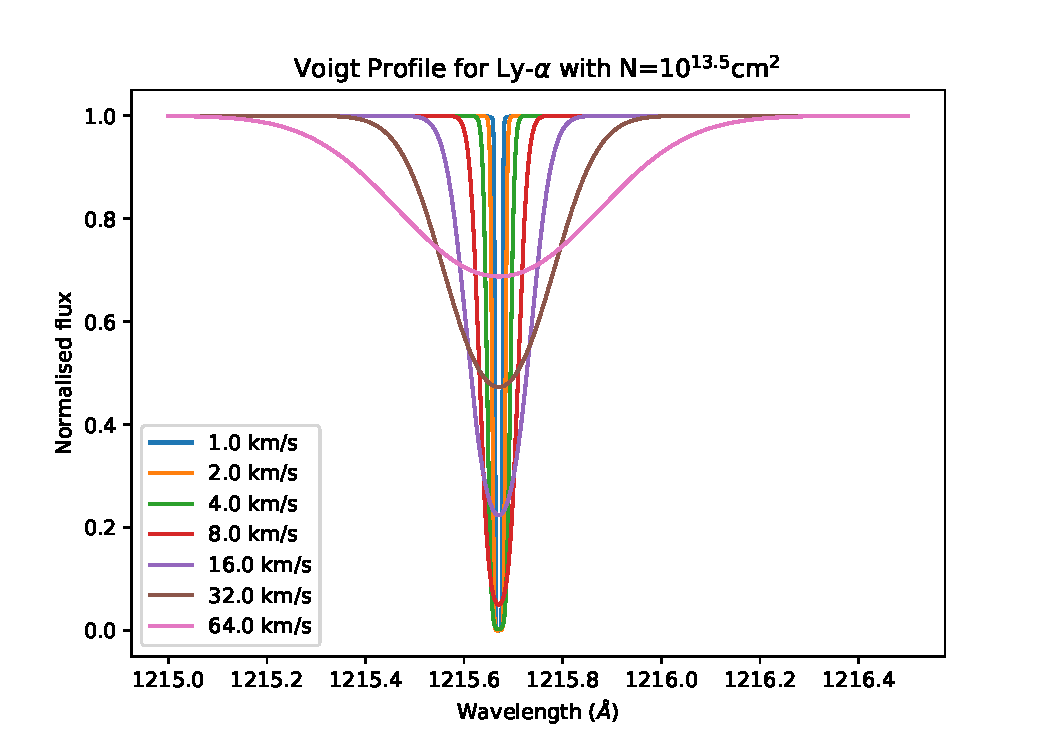
\includegraphics[width=1\linewidth]{../Voigt-Ly-a_vary_b}
\caption{Effect of b-parameter on the Voigt profile}
\label{fig:voigt-ly-a_vary_b}
\end{figure}

The parameter b is related to the temperature as $b \propto \sqrt{T}$. We can see that the line profile becomes broader with increasing temperatures but the central optical depth goes down.

\subsubsection{Effect of Column density:}

\begin{figure}[H]
\centering
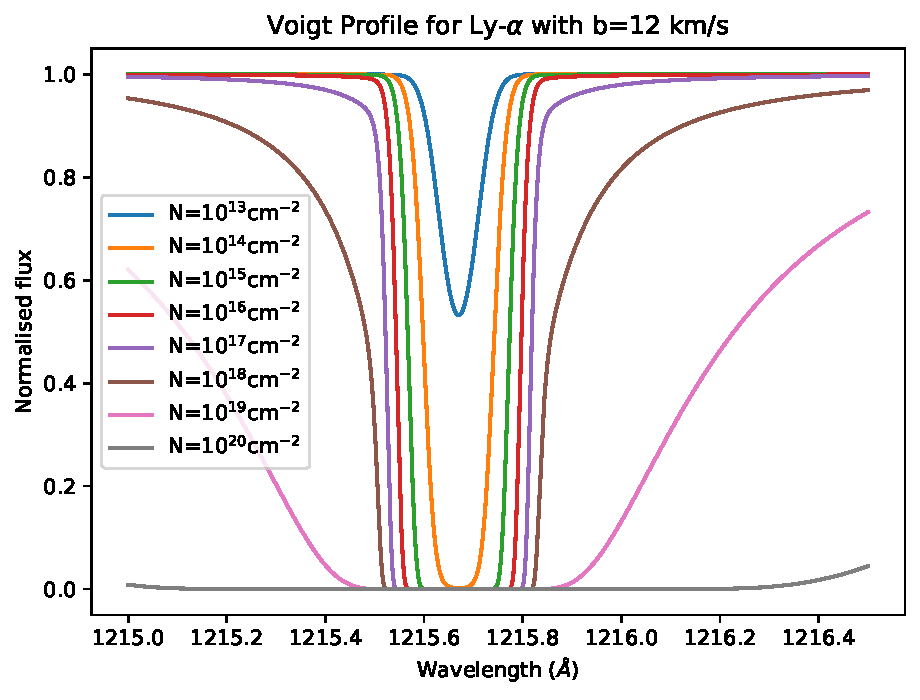
\includegraphics[width=1\linewidth]{../Voigt-Ly-a_vary_N}
\caption{Effect of column density N on the Voigt profile}
\label{fig:voigt-ly-a_vary_N}
\end{figure}

We can see that the line profile becomes broader with increasing column density and the central optical depth goes up. Hence we expect the equivalent width to strictly increase with respect to column density. We will soon check that in the next section.


%\cite{astropy:2013}

\subsection{Numerically generated Curve of Growth :}

The equivalent width in the wavelength domain can be computed as
\begin{align}
W_{\lambda} = \int_{0}^{\infty} [1 -\exp (-\tau_{\lambda})] d\lambda
\end{align}
This integrand peaks at $\lambda=\lambda_{12}$ and vanishes quickly, so we can approximate the above integral as
\begin{align}
W_{\lambda} = \int_{-\infty}^{\infty} [1 -\exp (-\tau_{\lambda})] d\lambda
\end{align}
Now we can define $\lambda' = \lambda - \lambda_{12}$ so that the integrand will be symmetric around $\lambda' = 0$. We can then use QUADPACK in SciPy to compute the equivalent width. QUADPACK chooses the best suited integration routine automatically. As an alternative we could use simple trapezoidal rule but that will require evaluating the Voigt function larger number of times and hence not a good idea.

\begin{figure}[H]
\centering
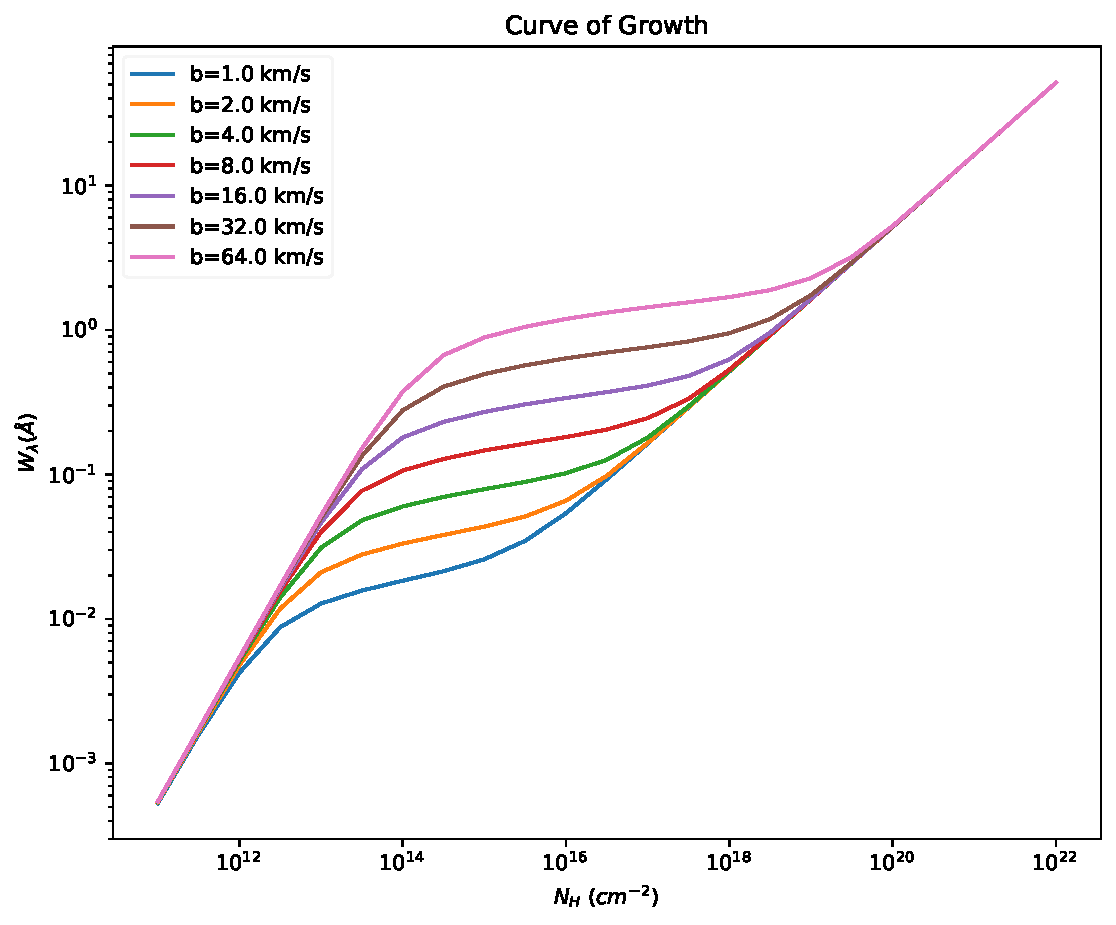
\includegraphics[width=1\linewidth]{../CoG_Ly-alpha}
\caption{Curve of growth for the Ly-$\alpha$ line}
\label{fig:cog-ly-alpha}
\end{figure}
In the figure \ref{fig:cog-ly-alpha}, we can see that in the log scale, $W_{\lambda}$ increases linearly with slope 1 for low column densities, this means $W_{\lambda} \propto N$ and this regime is identified as the linear regime. For high column densities the log plot is again linear but the slop is half, this means $W_{\lambda} \propto \sqrt{N}$, this is identified as the damped regime. In the intermediate regime, the equivalent width increases very slowly and it is not a power law, this is identified as the saturated regime. The column density range for each regime is dependent on the thermal parameter $b$. For $b = 64$km/s, we can see that the linear regime extends upto $N=10^{14}$ cm$^{-2}$, then the saturated regime goes upto $N=10^{21}$ cm$^{-2}$ and then the damped regime starts.\\


A slightly different plot is made for the curve of growth in \ref{fig:cog-ly-alpha_gen}, we will see its usefulness soon.

\begin{figure}[H]
\centering
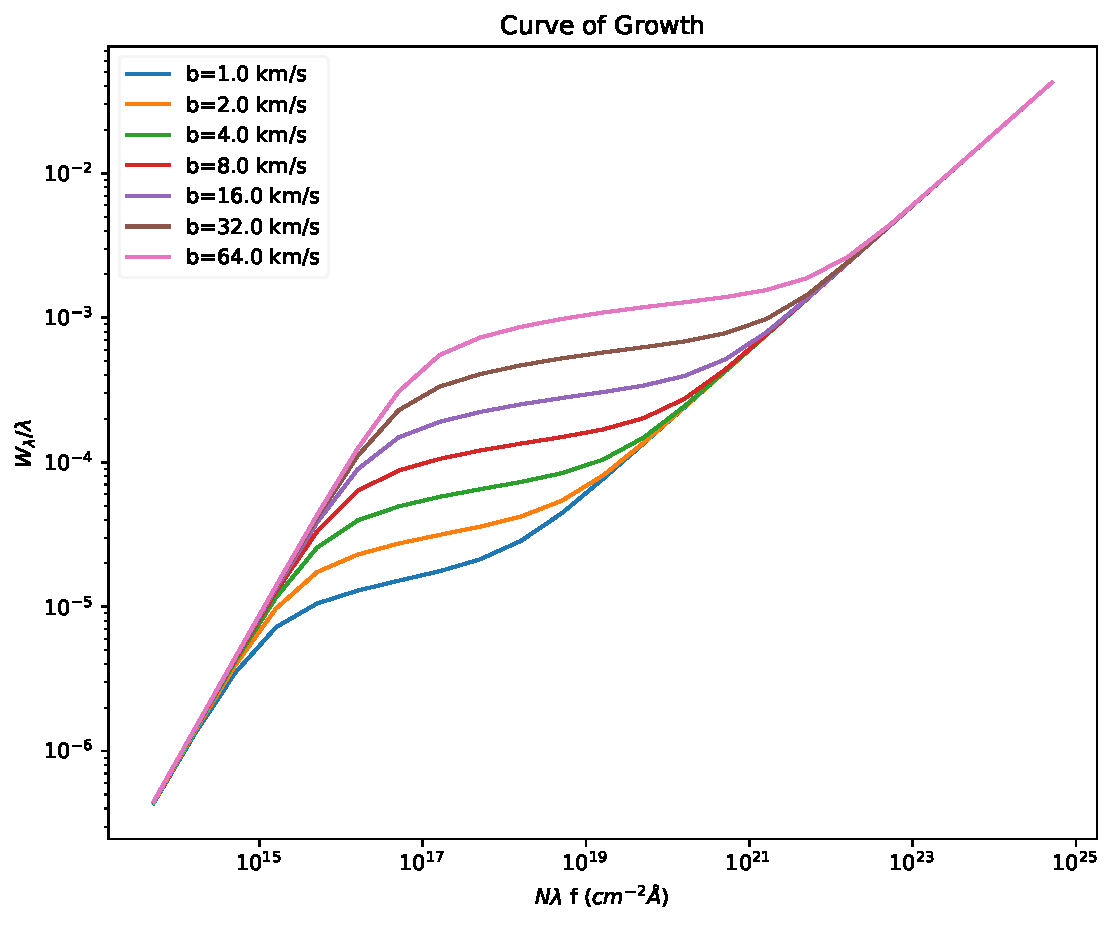
\includegraphics[width=1 \linewidth]{../CoG_Ly-alpha_gen}
\caption{Curve of growth for the Ly-$\alpha$ line [W/$\lambda$] vs [N$\lambda$f]}
\label{fig:cog-ly-alpha_gen}
\end{figure}




\subsection{Analytical approximation for Curve of Growth:}
\label{sec:approx}
We saw that the curve of growth can be explained simply by considering three different regimes of the column density.
In the linear regime we have,
\begin{align}
\frac{W_{\lambda}}{\lambda} = N \lambda f \left( \frac{\pi e^2}{mc^2} \right) 
\end{align}
In the saturated regime we have,
\begin{align}
\frac{W_{\lambda}}{\lambda} = 2 \frac{b}{c} \sqrt{\ln \left( \frac{\sigma_{0} N \lambda f}{b}\right) } \qquad \text{where} \quad \sigma_{0} = \left( \frac{\pi e^2}{mc} \right) 
\end{align}
In the damped regime we have,
\begin{align}
\frac{W_{\lambda}}{\lambda} = 2 \sqrt{ N \lambda f \left( \frac{\pi e^2}{mc^2} \right) \left( \frac{\gamma \lambda}{\pi^3c} \right)  }
\end{align}

\begin{figure}[H]
	\centering
	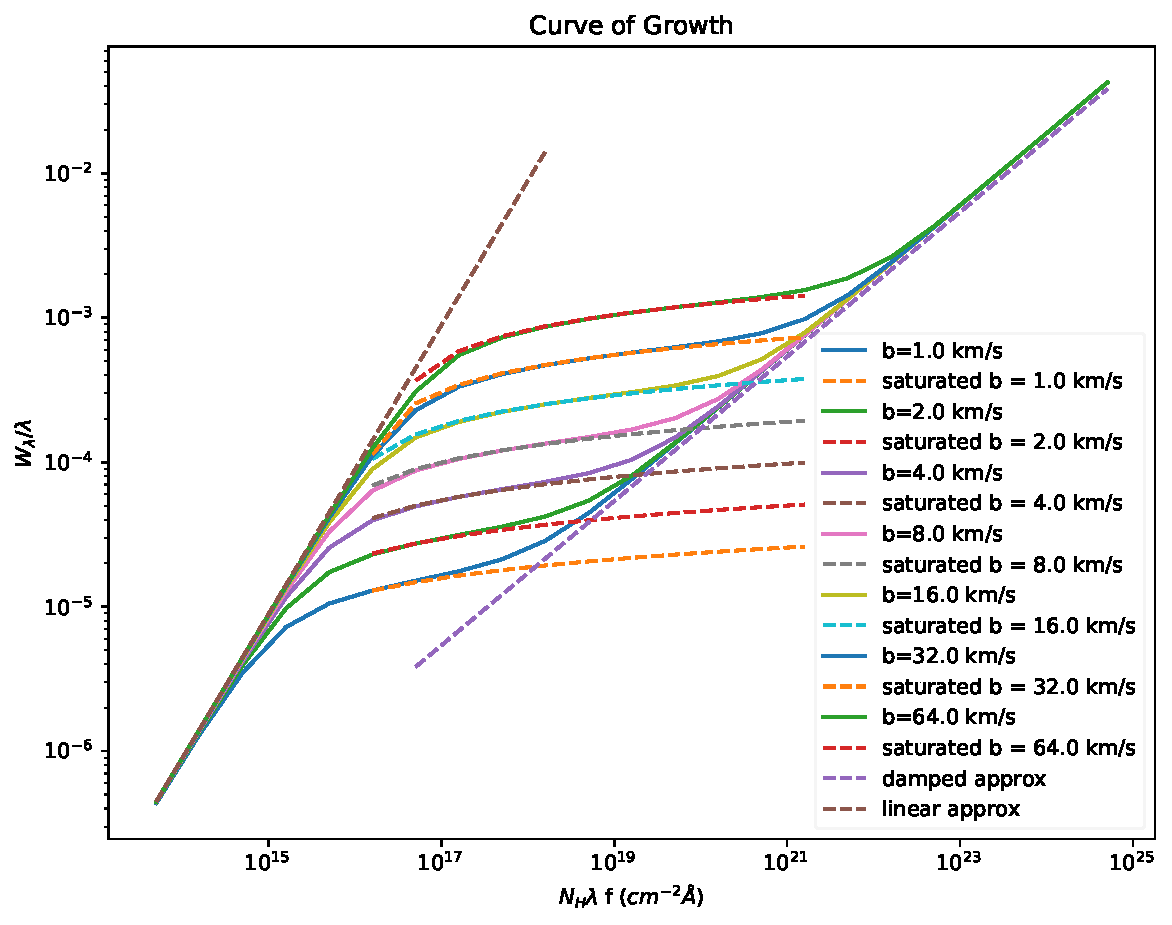
\includegraphics[width=1\linewidth]{../CoG_Ly-alpha-approx_gen}
	\caption{Comparison of exact numerical and analytical approximations for the curve of growth of the Ly-$\alpha$ line. [W/$\lambda$] vs [N$\lambda$f]}
	\label{fig:cogly-alpha-approxgen}
\end{figure}
In the figure \ref{fig:cogly-alpha-approxgen} we can see that the approximations matches very well within some regimes.

\newpage

\subsection{Uniqueness of the Curve of Growth:}
Now let us plot the curve of growth for different lines in different ions. 
\begin{figure}[H]
	\centering
	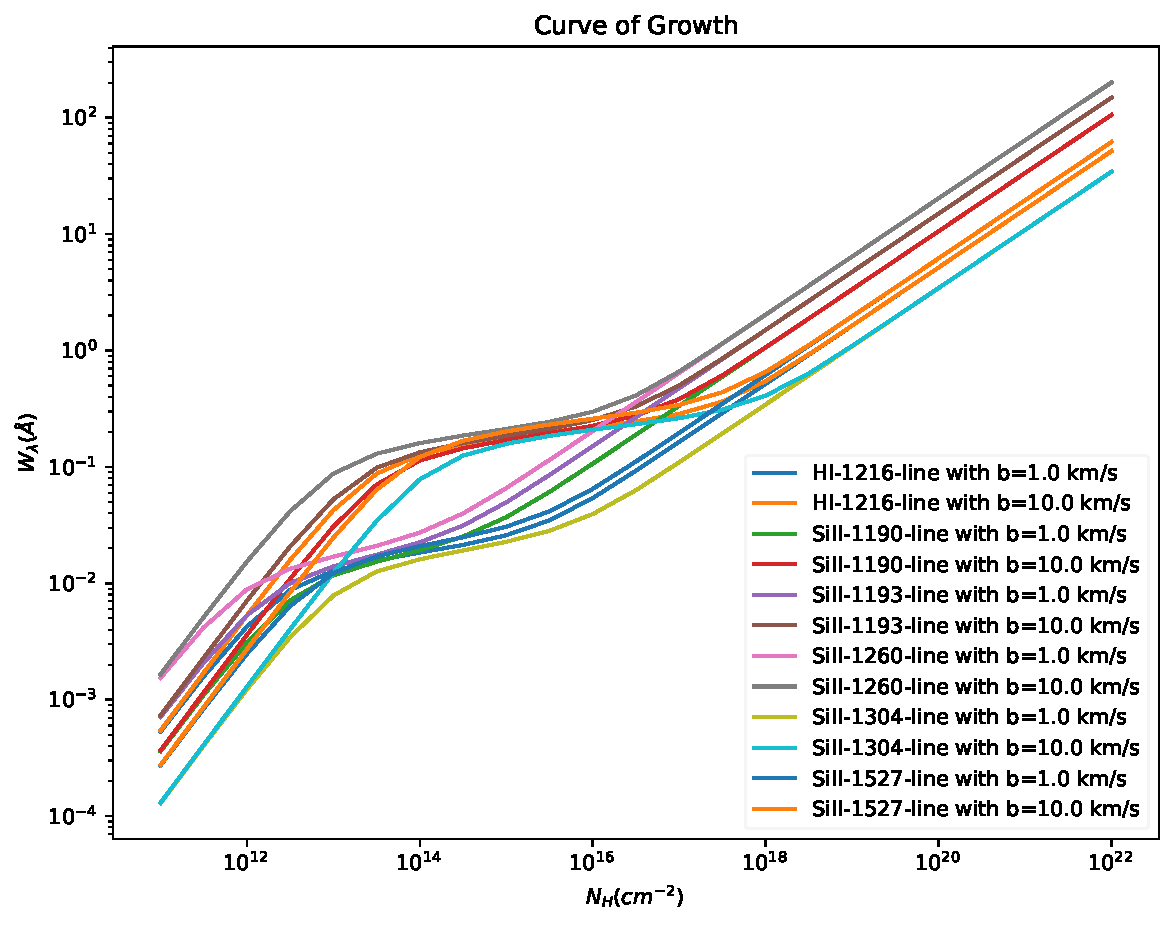
\includegraphics[width=1\linewidth]{../CoG_multi}
	\caption{Curve of growth for different lines}
	\label{fig:cog_multi}
\end{figure}
We can see in figure \ref{fig:cog_multi} that they are similar but differ by some factors. Now come the use of [W/$\lambda$] vs [N$\lambda$f] plot, as the curve does not depend on the transition line properties in both the linear and saturated regime. We can see  in the figure \ref{fig:cog_multi_gen} that for a given value of $b-parameter$, the curve is unique in linear and saturated regime.

\begin{figure}[H]
	\centering
	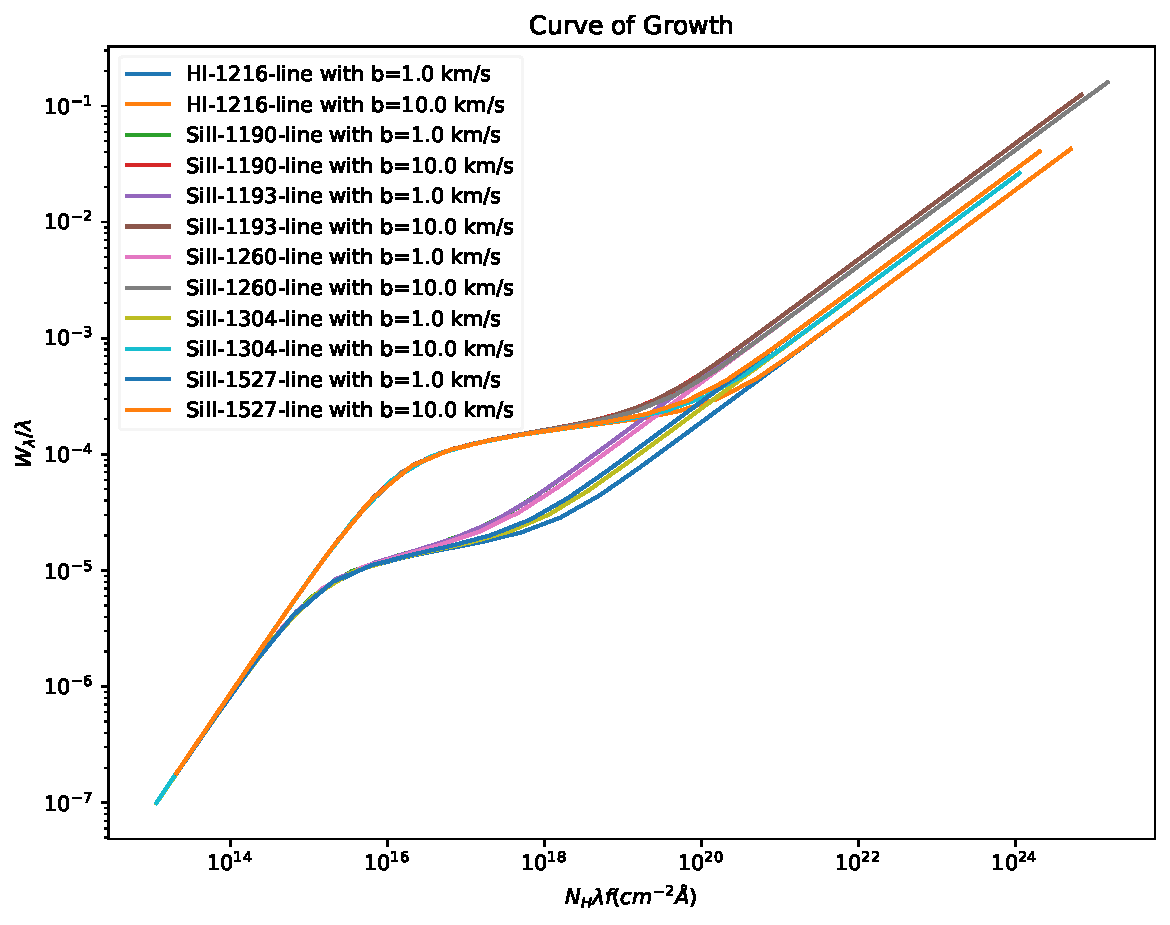
\includegraphics[width=1\linewidth]{../CoG_multi_gen}
	\caption{Curve of growth [W/$\lambda$] vs [N$\lambda$f] for different lines}
	\label{fig:cog_multi_gen}
\end{figure}




%voigt times
%17.452857494354248
% 0.005995750427246094
 

 
 
% \begin{figure}
% 	\centering
% 	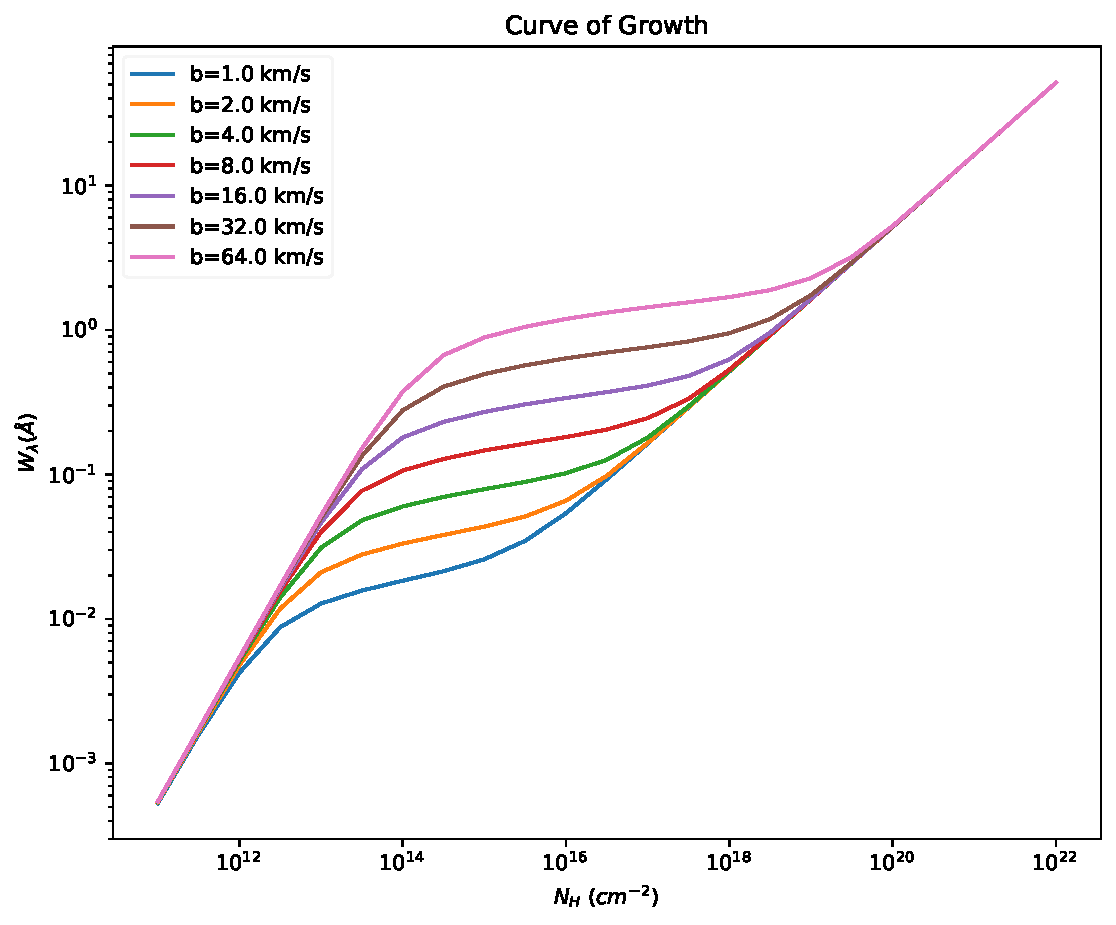
\includegraphics[width=0.9\linewidth]{../CoG_Ly-alpha}
% 	\caption{}
% 	\label{fig:cogly-alpha}
% \end{figure}
 
\newpage
 
\section{ISM lines}
In this section, we will study the absorption lines caused by ISM in a given quasar spectrum.

\subsection{Equivalent widths of the identified lines:}
\begin{itemize}
\item {The lines listed in the give atom.dat file is sorted according to the central wavelength.}
\item{The lines marked in green in the given pdf as ISM lines have been identified in the atom.dat}
\item{For lines of same ion, that are very close but have very different oscillation strength ($f$), the one with larger value of $f$ is considered.}
\item{A python class for Line is implemented and used to store line properties.}
\item{A child class called Line\_data is created for various methods to compute equivalent widths.}
\item{Trapezoidal  rule is used to compute equivalent width from the spectrum.}
\item{For overlapping lines the equivalent width is computed by integrating along one direction where there is no overlap and then multiplied it by two.}
\item{Computed equivalent widths are listed in the table in the next page.}%\ref{table:W}}

\end{itemize}
%Using the given atom.dat file, I have identified the marked lines and hence obtained  its parameters. 
%spectrum given in the file

%{“hlsp_igm_hst_cos_1es1553_g130m-g160m_v3_spec.dat”}



%\begin{table}[]
%\begin{tabular}{l|l|l|l}
%ID  &  Wavelength ($\AA$)& f & $\gamma (s^{-1})$ \\
%\hline
%AlII  & 1670.7886  & 1.74     & 1390000000 \\
%CI    & 1188.8329  & 0.0124   & 19500000   \\
%CI    & 1277.2452  & 0.0853   & 232000000  \\
%CI    & 1280.1352  & 0.0263   & 106000000  \\
%CI    & 1328.8333  & 0.0758   & 288000000  \\
%CI    & 1560.3092  & 0.0774   & 127000000  \\
%CI    & 1656.9284  & 0.149    & 360000000  \\
%CII   & 1334.5323  & 0.1278   & 288000000  \\
%CII*  & 1335.7077  & 0.115    & 288000000  \\
%CIV   & 1548.2049  & 0.1899   & 264200000  \\
%CIV   & 1550.77845 & 0.09475  & 262800000  \\
%FeII  & 1142.3656  & 0.00401  & 25600000   \\
%FeII  & 1143.226   & 0.0192   & 98100000   \\
%FeII  & 1144.9379  & 0.083    & 352000000  \\
%FeII  & 1608.45081 & 0.0577   & 274000000  \\
%FeII  & 1611.2005  & 0.00138  & 286000000  \\
%HI    & 1215.6701  & 0.4164   & 626500000  \\
%MgII  & 1239.9253  & 0.000632 & 1370000    \\
%MgII  & 1240.3947  & 0.000356 & 1540000    \\
%MnII  & 1197.184   & 0.1566   & 784000000  \\
%NI    & 1199.5496  & 0.132    & 407000000  \\
%NI    & 1200.2233  & 0.0869   & 402000000  \\
%NI    & 1200.7098  & 0.0432   & 400000000  \\
%NiII  & 1317.217   & 0.146    & 420500000  \\
%NiII  & 1370.132   & 0.0769   & 410000000  \\
%NiII  & 1454.842   & 0.0276   & 102000000  \\
%NiII  & 1502.148   & 0.006    & 39320000   \\
%NiII  & 1709.6042  & 0.0324   & 435000000  \\
%NiII  & 1741.5531  & 0.0427   & 500000000  \\
%NiII  & 1751.9157  & 0.0277   & 370000000  \\
%NV    & 1238.821   & 0.156    & 339100000  \\
%NV    & 1242.804   & 0.077    & 335600000  \\
%OI    & 1302.1685  & 0.048    & 565000000  \\
%PII   & 1152.818   & 0.245    & 1230000000 \\
%SII   & 1250.578   & 0.00543  & 46300000   \\
%SII   & 1253.805   & 0.0109   & 46200000   \\
%SII   & 1259.518   & 0.0166   & 46500000   \\
%SiII  & 1190.4158  & 0.292    & 4080000000 \\
%SiII  & 1193.2897  & 0.582    & 4070000000 \\
%SiII  & 1260.4221  & 1.18     & 2950000000 \\
%SiII  & 1304.3702  & 0.0863   & 1010000000 \\
%SiII  & 1526.70698 & 0.133    & 1130000000 \\
%SiIII & 1206.5     & 1.63     & 2480000000 \\
%SiIV  & 1393.76018 & 0.513    & 880000000  \\
%SiIV  & 1402.77291 & 0.254    & 862000000 
%\end{tabular}
%\end{table}


\begin{table}[H]
	\label{table:W}
	\begin{tabular}{l|l|l|l|l}
		ID  &  Wavelength ($\AA$)& f & decay rate $\gamma (s^{-1})$ & Equivalent width, W ($\AA$)\\
		\hline &&&&\\
		HI    & 1215.670 & 4.1640e-01 & 6.265e+08 & 12.4372 \\
		FeII  & 1144.938 & 8.3000e-02 & 3.520e+08 & 0.2888  \\
		FeII  & 1143.226 & 1.9200e-02 & 9.810e+07 & 0.1524  \\
		FeII  & 1142.366 & 4.0100e-03 & 2.560e+07 & 0.0631  \\
		FeII  & 1611.200 & 1.3800e-03 & 2.860e+08 & 0.0566  \\
		FeII  & 1608.451 & 5.7700e-02 & 2.740e+08 & 0.4903  \\
		NiII  & 1317.217 & 1.4600e-01 & 4.205e+08 & 0.0986  \\
		NiII  & 1370.132 & 7.6900e-02 & 4.100e+08 & 0.1055  \\
		NiII  & 1454.842 & 2.7600e-02 & 1.020e+08 & 0.0497  \\
		NiII  & 1502.148 & 6.0000e-03 & 3.932e+07 & 0.0168  \\
		NiII  & 1709.604 & 3.2400e-02 & 4.350e+08 & 0.0962  \\
		NiII  & 1741.553 & 4.2700e-02 & 5.000e+08 & 0.1434  \\
		NiII  & 1751.916 & 2.7700e-02 & 3.700e+08 & 0.0790  \\
		PII   & 1152.818 & 2.4500e-01 & 1.230e+09 & 0.1361  \\
		CI    & 1188.833 & 1.2400e-02 & 1.950e+07 & 0.0142  \\
		CI    & 1277.245 & 8.5300e-02 & 2.320e+08 & 0.0864  \\
		CI    & 1280.135 & 2.6300e-02 & 1.060e+08 & 0.0198  \\
		CI    & 1328.833 & 7.5800e-02 & 2.880e+08 & 0.0370  \\
		CI    & 1560.309 & 7.7400e-02 & 1.270e+08 & 0.0749  \\
		CI    & 1656.928 & 1.4900e-01 & 3.600e+08 & 0.1802  \\
		SiII  & 1190.416 & 2.9200e-01 & 4.080e+09 & 0.5445  \\
		SiII  & 1193.290 & 5.8200e-01 & 4.070e+09 & 0.5464  \\
		SiII  & 1260.422 & 1.1800e+00 & 2.950e+09 & 0.5559  \\
		SiII  & 1304.370 & 8.6300e-02 & 1.010e+09 & 0.2963  \\
		SiII  & 1526.707 & 1.3300e-01 & 1.130e+09 & 0.5508  \\
		MnII  & 1197.184 & 1.5660e-01 & 7.840e+08 & 0.0423  \\
		NI    & 1199.550 & 1.3200e-01 & 4.070e+08 & 0.3449  \\
		NI    & 1200.223 & 8.6900e-02 & 4.020e+08 & 0.4480  \\
		NI    & 1200.710 & 4.3200e-02 & 4.000e+08 & 0.2183  \\
		SiIII & 1206.500 & 1.6300e+00 & 2.480e+09 & 0.6704  \\
		NV    & 1238.821 & 1.5600e-01 & 3.391e+08 & 0.1435  \\
		NV    & 1242.804 & 7.7000e-02 & 3.356e+08 & 0.0755  \\
		MgII  & 1239.925 & 6.3200e-04 & 1.370e+06 & 0.0420  \\
		MgII  & 1240.395 & 3.5600e-04 & 1.540e+06 & 0.0330  \\
		SII   & 1250.578 & 5.4300e-03 & 4.630e+07 & 0.2114  \\
		SII   & 1253.805 & 1.0900e-02 & 4.620e+07 & 0.2319  \\
		SII   & 1259.518 & 1.6600e-02 & 4.650e+07 & 0.4181  \\
		OI    & 1302.168 & 4.8000e-02 & 5.650e+08 & 0.3129  \\
		CII   & 1334.532 & 1.2780e-01 & 2.880e+08 & 0.6838  \\
		CII*  & 1335.708 & 1.1500e-01 & 2.880e+08 & 0.2679  \\
		SiIV  & 1393.760 & 5.1300e-01 & 8.800e+08 & 0.5052  \\
		SiIV  & 1402.773 & 2.5400e-01 & 8.620e+08 & 0.2676  \\
		CIV   & 1548.205 & 1.8990e-01 & 2.642e+08 & 0.5996  \\
		CIV   & 1550.778 & 9.4750e-02 & 2.628e+08 & 0.4308  \\
		AlII  & 1670.789 & 1.7400e+00 & 1.390e+09 & 0.5659 \\
	\end{tabular}
\end{table}


\subsection{Lymen - $\alpha$ line}

The Lyman alpha line is very strong and its effect is noticeble over wide range of wavelengths. There are multiple other weak lines in that range. We can see that the automatically generated continuum plot in green, represents the Lymen alpha line very well. A constant value [$1.6 \times 10^{14}$] is assumed to be the real continuum. \\
Now by integrating that, we get equivalent width, $W = 12.4372 \AA$.
Using the damped regime approximation we get the column density, $N = 7.126 \times 10^{20} $cm$^{-2}$.\\

Using this value for column density, I have generated and overlayed a Voigt profile onto the spectrum for different value of thermal parameter, $b$. We can see in figure \ref{fig:voigt-ly-a_overlay}, that for many values of $b$, the Voigt profile is same and matches the spectrum.

 
\begin{figure}[H]
\centering
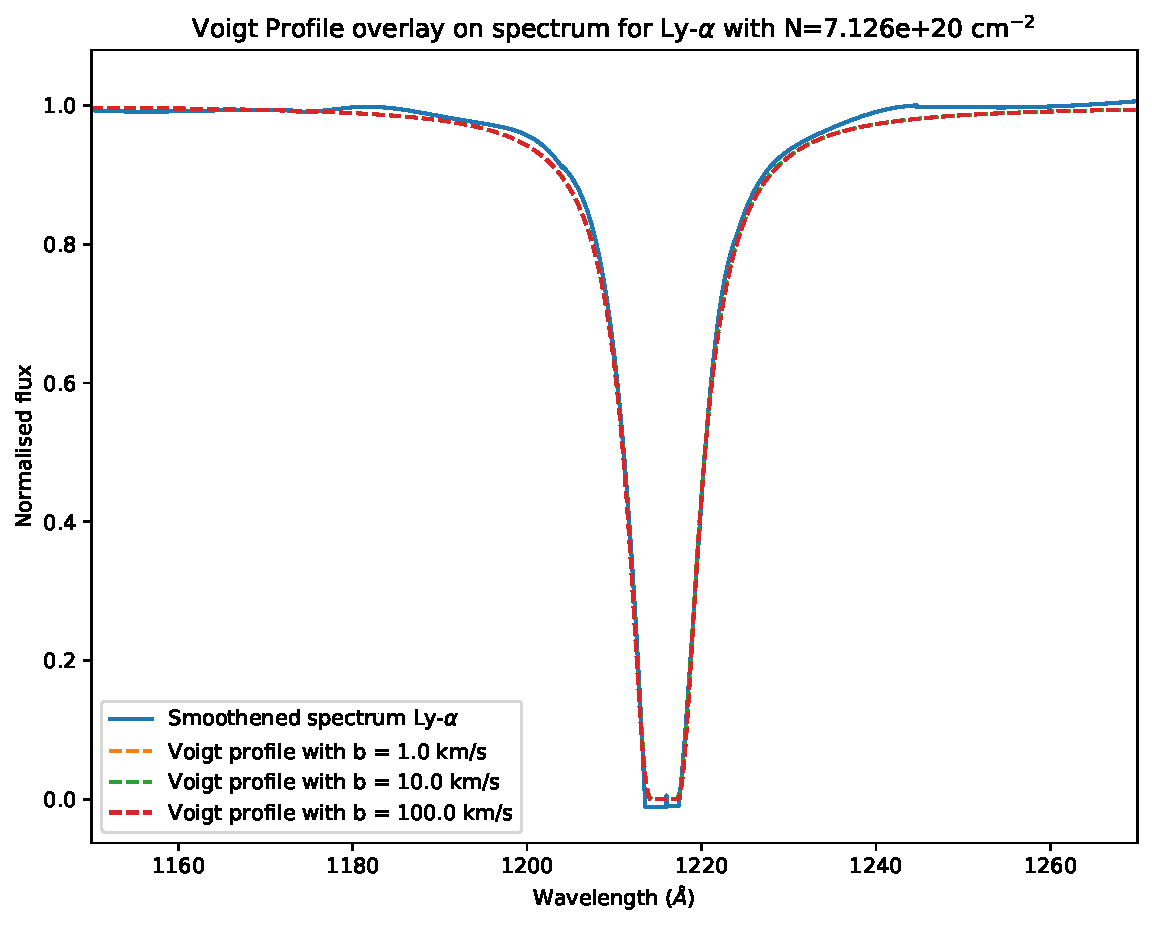
\includegraphics[width=0.9\linewidth]{../Voigt-Ly-a_overlay}
\caption{Overlay of Voigt profile guessed from the equivalent width using approximate relation in the damped regime.}
\label{fig:voigt-ly-a_overlay}
\end{figure}
 
\newpage 
\subsection{Fe II and Ni II in the ISM}
All the lines for FeII and NiII are in the linear or somewhat saturated regime. In that regime the curve of growth plotted as  [W/$\lambda$] vs [N$\lambda$f] does not depend on line transition parameters.
\begin{itemize}
\item{ I plotted [W/$\lambda$] vs [N$\lambda$f] curve for different values of $b$}
\item{I then scatter plotted the data for different values of $N$ onto the same axis.}
\item{By eyes I found the value of $b$ and $N$ at which the data is best fitted by the curve.}
\end{itemize}

By doing the above steps for only the Fe II lines, I obtained its column density to be $N=1.778 \times 10^{15}$cm$^{-2}$, and b value of 22 km/s.


\begin{figure}[H]
	\centering
	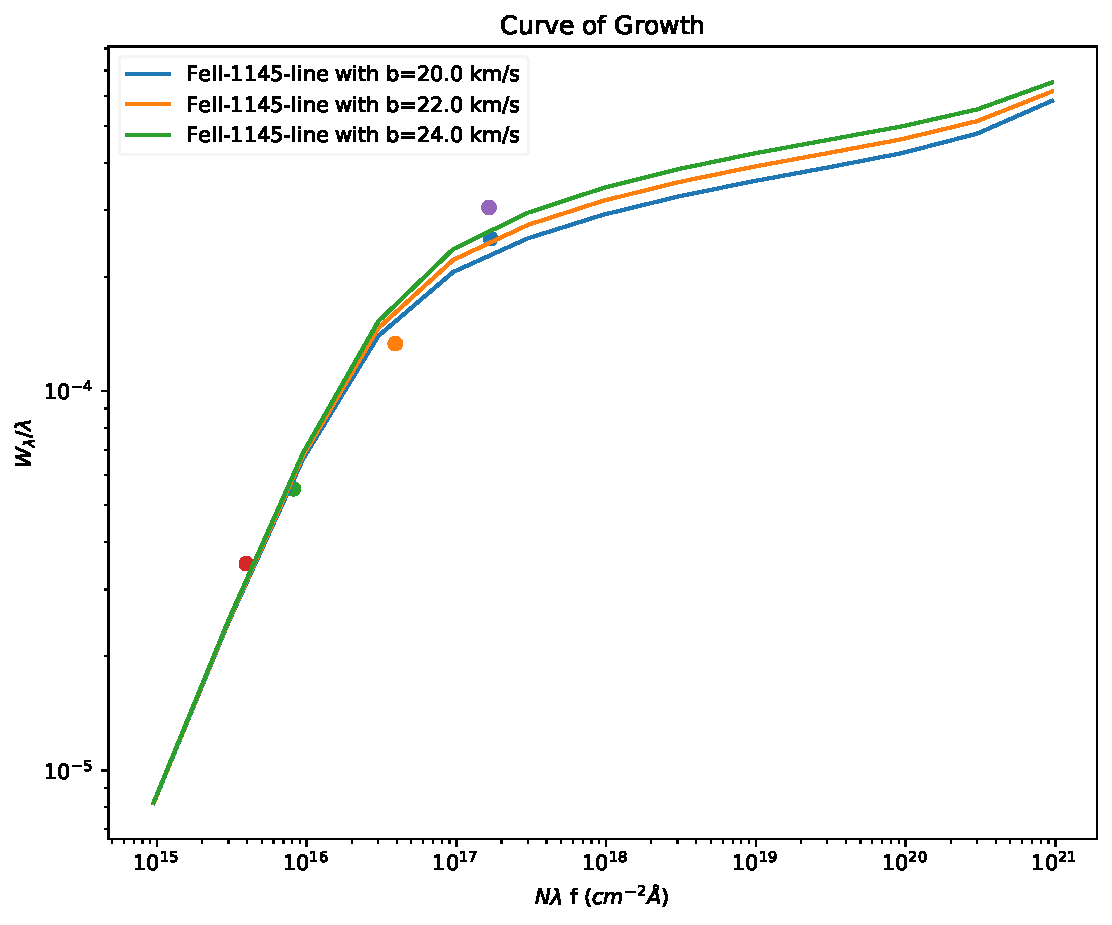
\includegraphics[width=0.9\linewidth]{../FeII-fiting}
	\caption{FeII fitting for $N=1.778 \times 10^{15}$cm$^{-2}$}
	\label{fig:feii-fiting}
\end{figure}

\newpage

By repeating the same procedure for only the Ni II lines, I obtained its column density to be $N=1.4 \times 10^{14}$cm$^{-2}$, and b value of 12 km/s.

\begin{figure}[H]
	\centering
	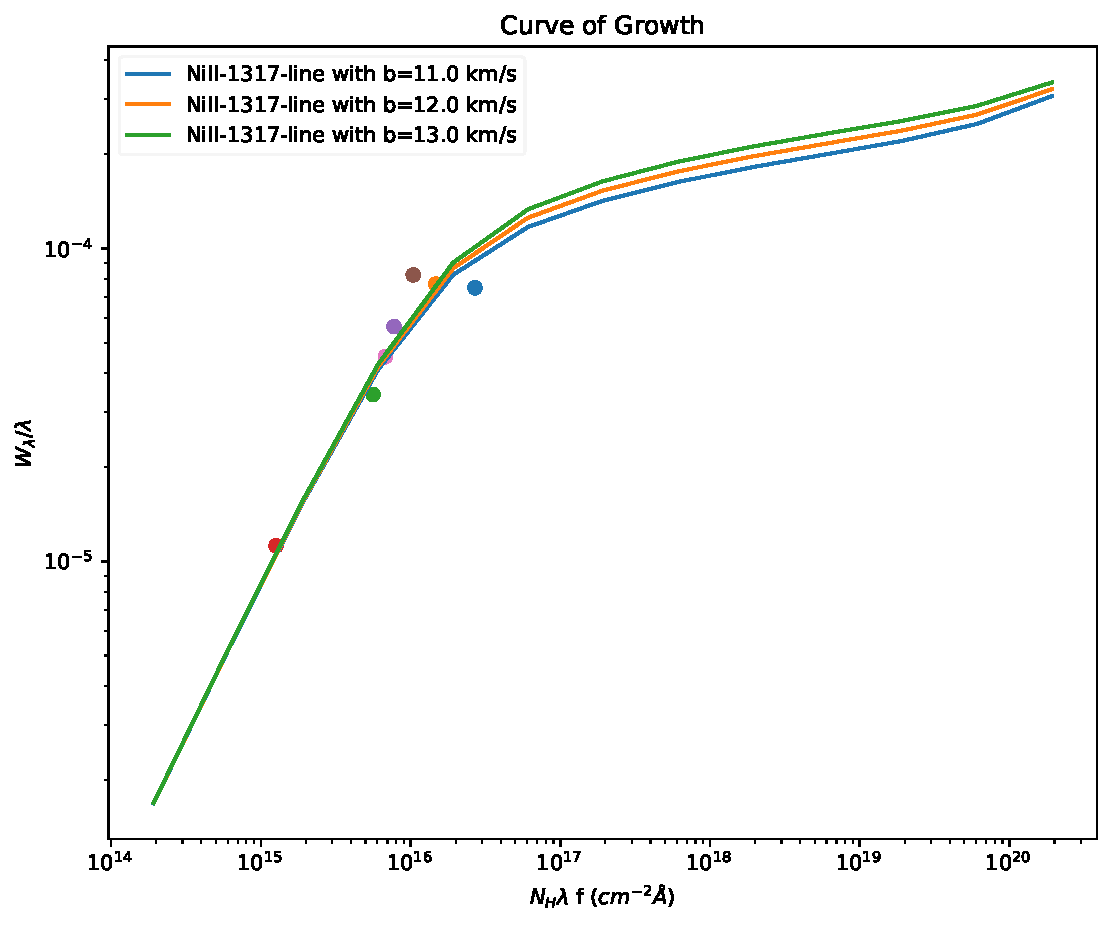
\includegraphics[width=0.9\linewidth]{../NiII-fiting}
	\caption{NiII-fitting for $N=1.4 \times 10^{14}$cm$^{-2}$}
	\label{fig:niii-fiting}
\end{figure}

\newpage

If we know somehow that the b-value has to be same, then we can get value by doing the above procedure for both the Fe II lines and the Ni II lines together. We can see that b value of 18 km/s  seems to fit both Fe II and Ni II.

\begin{figure}[H]
	\centering
	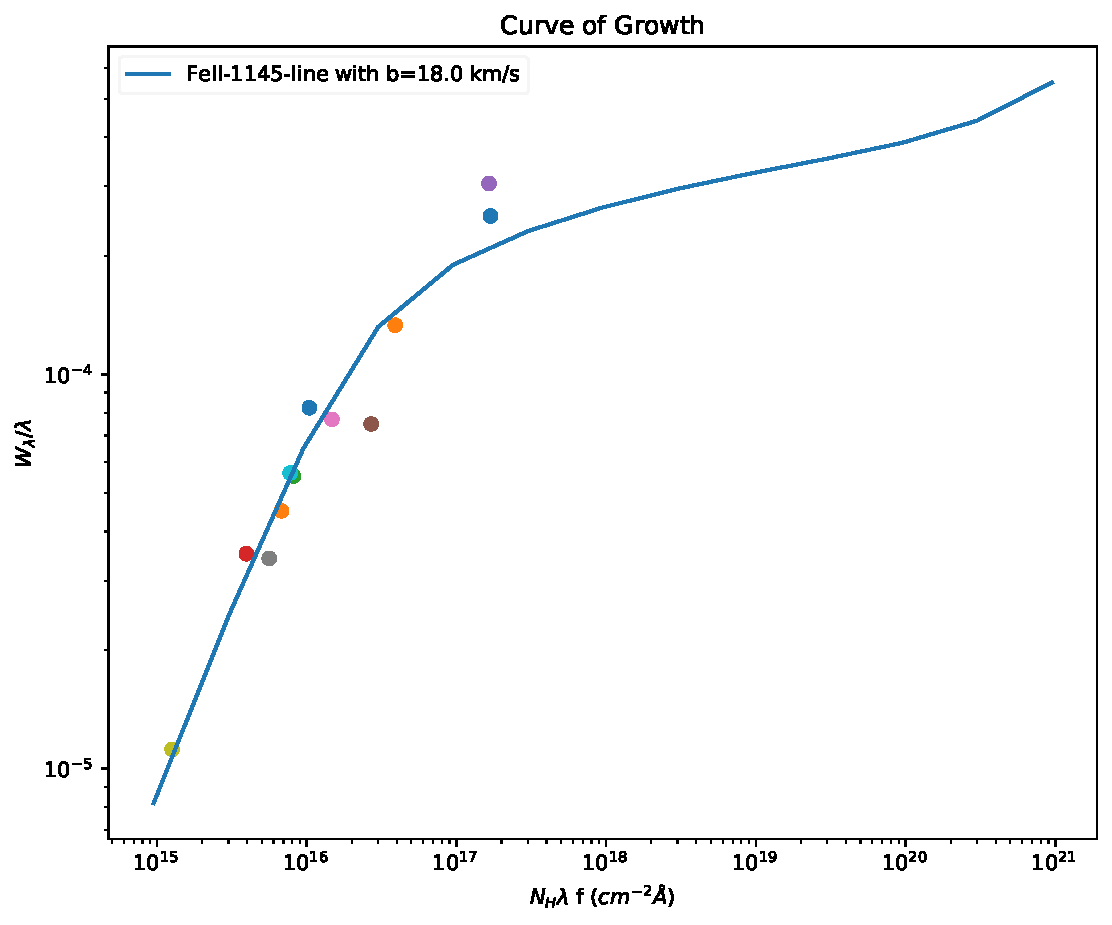
\includegraphics[width=0.9\linewidth]{../FeII-NiII-consist-fiting}
	\caption{Combined FeII and NiII fitting}
	\label{fig:feii-niii-consist-fiting}
\end{figure}

\newpage

\subsection{Column density table for all identified lines:}
By looking at the spectrum, it seems that most of the identified lines other than the HI, FeII and NiII lines are in the linear regime. Hence the column density can be obtained directly using the linear relation mentioned in section \ref{sec:approx}.
\begin{table}[H]
\begin{tabular}{l|l}
ID & Column density N (cm$^{-2}$)\\
\hline & \\
FeII  & 1.778e+15 \\
NiII  & 1.400e+14 \\
PII   & 4.721e+13 \\
CI    & 5.656e+13 \\
SiII  & 1.371e+14 \\
MnII  & 2.130e+13 \\
NI    & 3.351e+14 \\
SiIII & 3.192e+13 \\
NV    & 6.972e+13 \\
MgII  & 5.849e+15 \\
SII   & 2.044e+15 \\
OI    & 4.342e+14 \\
CII   & 3.394e+14 \\
CII*  & 1.475e+14 \\
SiIV  & 5.888e+13 \\
CIV   & 1.812e+14 \\
AlII  & 1.316e+13
\end{tabular}
\end{table}


 


%\bibliography{astropy}{}
%\bibliographystyle{plain}
\begin{thebibliography}{8}
	\bibitem{Voigt1D_comments}
	Comments on the Voigt function implementation in the Astropy andSpectraPlot.com packages ~\url{https://arxiv.org/pdf/1806.10338.pdf}
	\bibitem{Voigt1D-bug}
	Bug in Voigt1D provided by astropy
	\url{https://github.com/astropy/astropy/issues/7256}
	\bibitem{scipython}
	\url{https://scipython.com/book/chapter-8-scipy/examples/the-voigt-profile/}
\end{thebibliography}


\end{document}